\chapter{图表}
\label{chap:fig_tab}

用LaTex插入图表的最大优势在于交叉引用十分方便。LaTex中,章节、图表、公式的交叉引用都是通过\texttt{\string\label}和\texttt{\string\ref}命令实现的。以下是插入图表的示例,以及可能存在的问题。

\section{图}

用LaTex插入图片可以插入png/jpg格式的像素图,也可以插入pdf格式的矢量图(以\texttt{copy.tex}和\texttt{origin.tex}为例)。以北大word模板中的图片示例如下:

\begin{figure}[!htbp]
    \centering
    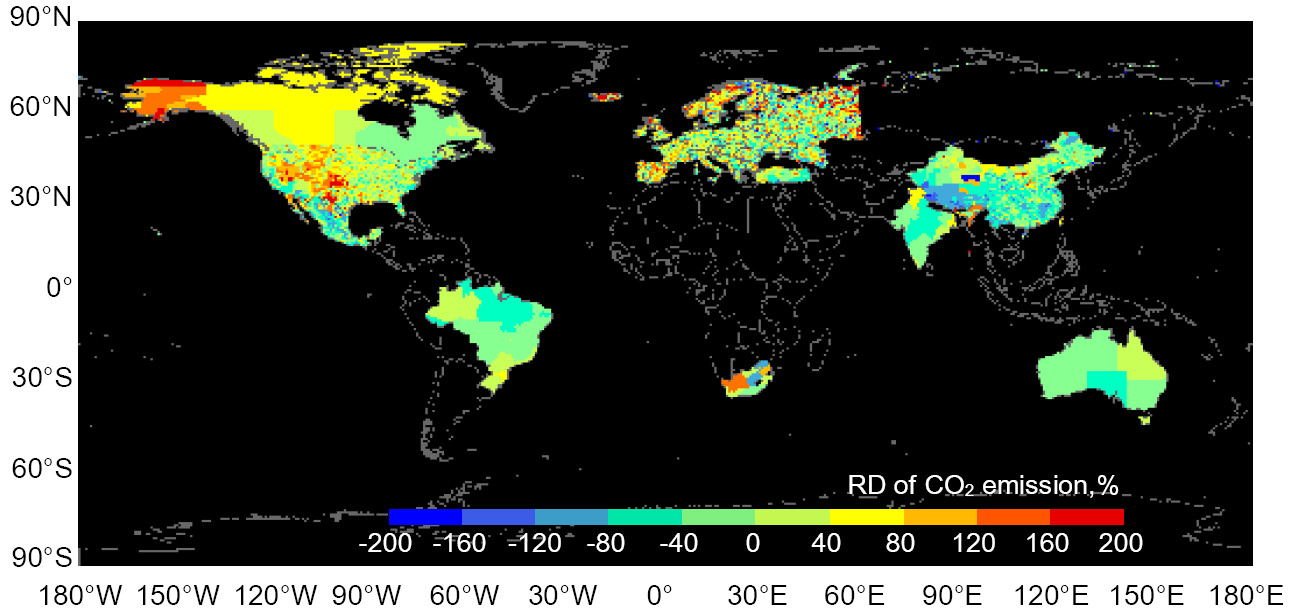
\includegraphics[width=0.8\linewidth]{img/ch3/fig_example.png}  %width控制图片宽度占行宽的比例
    \caption{全球NAT-CO2-2007清单与PKU-CO2-2007比较的空间示意图}         %caption的位置决定了标题出现在图表上方或下方
    \label{fig:fig_example}
\end{figure}

\section{表}

用北大word模板中的表格作为例子,插入表格示例如下:

\begin{table*}[!htbp]
\centering
\caption{室外细菌气溶胶香农-维纳指数(H)和均匀性指数(E)\protect\footnotemark[1]}    %注意脚注命令footnotemark,以及\protect命令,表示修正,使其后的代码被识别为命令而非表格的标签
\label{tab:table_example}
\renewcommand\arraystretch{1.6} %控制表格中的行距
\begin{tabular}{ccccccccccccc}  %c表示设置单元格居中,如果是 l 或 r 则分别为左对齐或右对齐
\Xhline{1.5pt}
\multirow{1}{*}{}   & \multicolumn{4}{c}{\textbf{Stage 1 (>7.1 μm)}}   & \multicolumn{4}{c}{\textbf{Stage 2 (4.8-7.1 μm)}} &  \multicolumn{4}{c}{\textbf{Stage 3 (3.2-4.7 μm)}}    \\  
\cline{2-13}
 &  Con &  Low &  Medium &  High &  Con &  Low &  Medium &  High &  Con &  Low &  Medium &  High  \\
 \hline
\textbf{H} &  \textbf{2.52} &  2.58 &  2.57 &  \textbf{\textit{2.24}} &  \textbf{2.48} &  2.21 &  2.21 &  \textbf{\textit{2.36}} &  \textbf{2.66} &  2.65 &  2.64 &  2.53 \\
\textbf{E} &  0.87 &  0.88 &  0.93 &  0.85 &  0.9 &  0.86 &  0.86 &  0.85 &  0.9 &  0.9 &  0.85 &  0.88 \\ 

\Xhline{1.5pt}
\end{tabular}
\end{table*}

\footnotetext[1]{这里做一个脚注的例子。同时指出,该示例表格宽度超过了行宽,会使得编译时警告,且排版出的表格不够漂亮。使用者如遇类似情况可自行查询LaTex用法,减小宽度、表格居中或页面横置,以使得排版美观。}

\section{问题}

\subsection{交叉引用时的空格问题}

引用章节、图表或公式,都会遇到一个问题,即编号的阿拉伯数字和前后文字距离过近,排版时很不好看,需要手动添加空格或者公式环境下的波浪符号(LaTex会编码为空格)以隔开。例如:图\ref{fig:fig_example}表明、图 \ref{fig:fig_example} 表明、图$~$\ref{fig:fig_example}$~$表明,就可以看出区别。使用者可自行调整。

\subsection{长表格和表格注释}

本人论文写作中遇到两个问题。其一是长表格问题,可以通过\texttt{longtable}环境解决。其二是对表格的某些单元格添加表注,可以通过在表格下方添加注释,或者在页面下方添加脚注的方式解决。这些问题并不复杂,如遇到请使用者自行查询。另,pkuthss v1.9.4模板中有这两个问题的例子,可参考其代码。

\subsection{图表位置问题}

查看示例代码可发现,图表位置的设置为\texttt{[!htbp]},意为按照“当前位置、页面顶部、页面底端和另一页搜寻最优位置”四种方式依次选取合适的位置放置图表。但是,排版时可能出现图表位置不美观的情况,使用者可以通过在源代码中调整插入图表代码的位置,或者改变图表位置的设置解决。